\documentclass[11pt,twocolumn]{article}
\usepackage[utf8]{inputenc}
\usepackage[T1]{fontenc}
\usepackage{amsmath,amssymb,amsfonts}
\usepackage{booktabs}
\usepackage{graphicx}
\usepackage{hyperref}
\usepackage{xcolor}
\usepackage[margin=2cm]{geometry}
\usepackage{authblk}
\usepackage{multirow}

\title{Non-Associative Curvature of Octonion State-Space Models\\
as Interpretable Biomarker of Path-Dependent Neural Dynamics}

\author[1]{Demetrios Brinkmann}
\affil[1]{Sounio Project}

\date{\today}

\begin{document}
\maketitle

%% F10: Abstract reformulated to match evidence (proof-of-concept framing)
\begin{abstract}
State-space models (SSMs) with hypercomplex recurrence operators encode multi-dimensional temporal dynamics, but interpreting \emph{what} the learned operator captures remains an open problem. We introduce a Hessian-based diagnostic that measures the off-diagonal curvature of the binary cross-entropy loss landscape with respect to the octonion recurrence parameter $A \in \mathbb{O}$ of an Octonion SSM (O-SSM). Because octonion multiplication is non-associative, the off-diagonal Hessian norm $\|H_{\mathrm{od}}\|_1$ can detect, in individual patients, the degree to which the trained model exploits path-dependent state evolution---a property absent in associative algebras. We evaluate this diagnostic on two EEG datasets: (i)~the CHB-MIT Scalp EEG Database (7 patients with ictal data from a cohort of 9) and (ii)~the EEGMMIDB motor imagery corpus (30 subjects). On CHB-MIT, 2 of 5 evaluable patients show statistically significant two-sided separation between ictal and baseline off-diagonal curvature (P3 chb03: two-sided $p{=}0.06$; P6 chb10: two-sided $p{=}0.05$; $n{=}1000$ shuffles), indicating that the Hessian diagnostic captures seizure-state changes in the loss landscape. Notably, the direction of difference is not uniform: most patients show baseline $>$ ictal, suggesting that the Hessian norm indexes a \emph{state change} rather than a directional increase. On EEGMMIDB, task conditions show 9.2\% higher off-diagonal curvature than rest ($p{=}0.04$ by bootstrap). Across both datasets, O-SSM consistently produces higher off-diagonal norms than a quaternion control (H-SSM), confirming that the extra curvature arises from non-associativity rather than dimensionality. We release all code in the Sounio language for reproducibility. This work constitutes a proof-of-concept for non-associative Hessian diagnostics in neural time-series.
\end{abstract}

\section{Introduction}

Cortical signal propagation during seizures is inherently path-dependent: the order in which neural populations activate affects downstream dynamics \cite{lopes2003model}. Standard recurrent models and SSMs use associative algebras (real, complex, quaternion) for their recurrence operators, which means the grouping of sequential operations does not affect the outcome. This makes them blind to associativity-sensitive temporal structure.

Octonions ($\mathbb{O}$), the largest normed division algebra, are non-associative: $(a \otimes b) \otimes c \neq a \otimes (b \otimes c)$ in general \cite{baez2002octonions}. An Octonion SSM (O-SSM) with recurrence $h_{t+1} = (A \otimes h_t) \otimes x_t$ therefore encodes path-dependent dynamics that an associative model cannot express.

The central question is: \emph{can we measure whether a trained O-SSM actually uses this non-associative capacity, and does it correlate with neurobiologically meaningful dynamics?}

We propose the \textbf{Hessian off-diagonal $L_1$-norm} as a diagnostic. The $8 \times 8$ Hessian of the loss $\mathcal{L}$ with respect to the octonion parameter $A$ captures second-order coupling between octonion components. Its off-diagonal entries measure cross-component curvature---precisely the interactions governed by the Fano plane that define octonion non-associativity. We provide proof-of-concept evidence that:

\begin{enumerate}
    \item In evaluable patients, the off-diagonal norm significantly \emph{separates} ictal from baseline EEG (two-sided permutation test), indicating the loss landscape occupies a different curvature regime during seizures;
    \item It decomposes into 7 interpretable Fano lines corresponding to specific electrode coupling paths;
    \item It is consistently higher in O-SSM than in a quaternion control (H-SSM), confirming the non-associative origin.
\end{enumerate}

\section{Background}

\subsection{Octonion Algebra and the Fano Plane}

The octonions $\mathbb{O}$ are an 8-dimensional algebra over $\mathbb{R}$ with basis $\{e_0, e_1, \ldots, e_7\}$, where $e_0 = 1$. Multiplication is defined by the Fano plane: a projective plane of order 2 with 7 points and 7 lines, each line containing 3 points \cite{baez2002octonions}. For any Fano line $(e_i, e_j, e_k)$, we have $e_i \cdot e_j = e_k$ (with sign determined by orientation).

The \textbf{associator} $[a,b,c] = (a \cdot b) \cdot c - a \cdot (b \cdot c)$ is zero for any associative algebra but generically non-zero for octonions. The associator vanishes when $a,b,c$ lie in any quaternionic subalgebra, but is non-zero when all 7 imaginary directions are involved.

\subsection{State-Space Models}

A discrete-time SSM with state $h_t \in \mathbb{R}^d$, input $x_t \in \mathbb{R}^d$, and recurrence matrix $A$ evolves as:
\begin{equation}
    h_{t+1} = A h_t + B x_t, \quad y_t = C h_t + D x_t.
\end{equation}
Recent work (S4 \cite{gu2022efficiently}, Mamba \cite{gu2023mamba}) has shown that structured $A$ matrices enable long-range temporal modeling. Hypercomplex SSMs replace real matrix multiplication with algebra-specific products \cite{parcollet2020survey,gaudet2018deep}.

\subsection{O-SSM: Octonion Recurrence}

The O-SSM uses octonion multiplication for state transition. Concretely, we define a \textbf{blended} update that combines both parenthesizations:
%% F5: Document actual state update formula
\begin{equation}
    h_{t+1} = (A \otimes h_t) \otimes x_t + \beta \cdot A \otimes (h_t \otimes x_t),
    \label{eq:blend}
\end{equation}
where $\beta = 0.2$ is the blending coefficient. \textbf{Note on parameter provenance:} $\beta = 0.2$ was adopted from a single-patient analysis of chb03 (MSE-ratio criterion, Door~III). Subject-stratified re-analysis across 7 CHB-MIT patients using $h_\mathrm{sep} = \|h_\mathrm{II} - h_\mathrm{IC}\|$ as the optimality criterion yields individual optima $\alpha^*_i$ with posterior mean $\hat{\mu} = 0.471$ and $\hat{\sigma} = 0.344$ (95\%~CI $= [0.153, 0.789]$); zero of seven subjects have $\alpha^* = 0.20$ as their individual optimum, and $P(\mu \in [0.18, 0.22]) = 0.018$. The value $\beta = 0.2$ is therefore a default chosen for reproducibility with prior results, not a population optimum. Clinically, $\beta$ should be treated as a patient-specific nuisance parameter. The first term is the ``left-associated'' product; the second is the ``right-associated'' product. When the algebra is associative (quaternions), these are identical and the blend reduces to $1.2 \cdot A \otimes h_t \otimes x_t$. For octonions, the difference between the two terms is precisely the associator $[A, h_t, x_t]$, making the blend sensitive to path-dependent dynamics.

\section{Method}

\subsection{Architecture}

%% F6: Clarified parameter count
The O-SSM processes a sequence of $T=8$ timesteps, each with $d=8$ input dimensions (one per octonion component). The state $h_t \in \mathbb{O}$ is initialized to $(1,0,\ldots,0)$. After processing all timesteps, a linear head produces a binary logit:
\begin{equation}
    \hat{y} = \sigma\left(\sum_{i=0}^{7} W_i \cdot h_T^{(i)} + w_a \cdot \bar{\alpha} + b\right),
\end{equation}
where $\bar{\alpha} = \frac{1}{T}\sum_t \|[A, h_t, x_t]\|$ is the mean associator norm.

The model has \textbf{18 parameters}: $A \in \mathbb{O}$ (8 components, trained), $W \in \mathbb{R}^8$ (8 weights), $w_a$ (1 associator weight), and $b$ (1 bias). All 18 are optimized (see Section~\ref{sec:training}).

\subsection{Training Protocol}
\label{sec:training}

The loss function is binary cross-entropy:
\begin{equation}
    \mathcal{L} = -\left[y \log p + (1 - y) \log (1 - p)\right],
\end{equation}
where $p = \sigma(\hat{y})$ and $y \in \{0, 1\}$ indicates ictal ($y=1$) vs.\ non-ictal ($y=0$). Training proceeds in two phases:
\begin{enumerate}
    \item \textbf{Head training} (60 epochs): $W$, $w_a$, $b$ are updated by SGD with momentum 0.9, learning rate 0.02. $A$ is held fixed.
    \item \textbf{Joint fine-tuning} (20 epochs): $A$ is updated via numerical gradient descent (central finite differences, step $\epsilon_g = 0.005$, learning rate 0.005) with re-normalization to $\|A\| = 1$ after each step. $W$, $w_a$, $b$ continue updating simultaneously.
\end{enumerate}

\subsection{Hessian Diagnostic}

%% F3: Corrected Eq. for H_ij to match code (standard 4-point formula)
After training, we compute the $8 \times 8$ Hessian matrix of the loss with respect to the 8 components of $A$ via central finite differences:
\begin{equation}
    H_{ii} = \frac{\mathcal{L}(A + \epsilon e_i) - 2\mathcal{L}(A) + \mathcal{L}(A - \epsilon e_i)}{\epsilon^2},
\end{equation}
\begin{equation}
    H_{ij} = \frac{f_{++} - f_{+-} - f_{-+} + f_{--}}{4\epsilon^2}, \quad i \neq j,
    \label{eq:hij}
\end{equation}
where $f_{++} = \mathcal{L}(A + \epsilon e_i + \epsilon e_j)$, $f_{+-} = \mathcal{L}(A + \epsilon e_i - \epsilon e_j)$, $f_{-+} = \mathcal{L}(A - \epsilon e_i + \epsilon e_j)$, $f_{--} = \mathcal{L}(A - \epsilon e_i - \epsilon e_j)$, with $\epsilon = 0.01$.

The \textbf{off-diagonal $L_1$-norm} is:
\begin{equation}
    \|H_{\mathrm{od}}\|_1 = \sum_{i \neq j} |H_{ij}|.
\end{equation}

For the quaternion control (H-SSM), only the $4 \times 4$ upper-left subblock is used.

\subsection{Fano-Line Decomposition}

We decompose $\|H_{\mathrm{od}}\|_1$ into 7 Fano lines, each contributing 6 off-diagonal entries ($|H_{ij}| + |H_{ji}|$ for 3 pairs):
\begin{align*}
    L_0 &= (e_1, e_2, e_4), \quad L_1 = (e_2, e_3, e_5), \\
    L_2 &= (e_3, e_4, e_6), \quad L_3 = (e_4, e_5, e_7), \\
    L_4 &= (e_5, e_6, e_1), \quad L_5 = (e_6, e_7, e_2), \\
    L_6 &= (e_7, e_1, e_3).
\end{align*}

When mapped to EEG channels (FP1-F7, F7-T7, FP2-F8, F8-T8, FP1-F3, F3-C3, FP2-F4, F4-C4), each Fano line captures specific inter-electrode coupling. \textbf{Caveat:} the assignment of channels to octonion components is fixed a priori; permuting this assignment would change the neuroanatomical interpretation. Future work should explore data-driven assignments.

\subsection{Permutation Test}

For each patient, we compute the observed difference $\Delta = \bar{H}_{\mathrm{od}}^{\mathrm{ictal}} - \bar{H}_{\mathrm{od}}^{\mathrm{baseline}}$ (in log-space). We then shuffle ictal/baseline labels 1000 times and compute $\Delta^*$ for each permutation. We report the \textbf{two-sided} $p$-value: $p_2 = |\{k : |\Delta^*_k| \geq |\Delta|\}| / 1000$. The two-sided test is appropriate because the Hessian diagnostic detects a \emph{state change} in the loss landscape rather than a directional increase.

\section{Experiments}

\subsection{CHB-MIT Seizure EEG}

\textbf{Dataset.} The CHB-MIT Scalp EEG Database \cite{shoeb2010application} contains continuous scalp EEG from 23 pediatric patients with intractable seizures, sampled at 256~Hz. We selected 9 patients (chb01, chb02, chb03, chb04, chb05, chb06, chb09, chb10, chb11), of which 7 have ictal data (chb04 and chb09 are baseline-only and excluded from main analyses).

%% F7: Removed patients without ictal data from main text
\textbf{Preprocessing.} Eight bipolar channels covering bilateral fronto-temporal pathways were extracted. Signals were z-normalized per channel per recording. Non-overlapping windows of 8 timesteps ($\approx$31~ms at 256~Hz) were extracted from ictal, interictal, pre-ictal (30~s before onset), post-ictal (30~s after end), and baseline (seizure-free file) segments.

\textbf{Protocol.} Leave-one-patient-out cross-validation: for each fold, one patient is held out, the model is trained on the rest, and the Hessian is computed on each held-out window.

Total: 3780 windows across 9 patients (7 with ictal data).

\subsection{EEGMMIDB Motor Imagery}

\textbf{Dataset.} 30 subjects from the EEG Motor Movement/Imagery Dataset \cite{schalk2004bci2000}, with rest (eyes open, R01) and task (motor imagery, R03) conditions.

\textbf{Preprocessing.} 8 channels, 8-timestep windows, z-normalized. 10-fold cross-validation.

Total: 800 windows (400 task, 400 rest).

\section{Results}

%% F7: Tables now show only 7 patients with ictal data (chb04/chb09 baseline-only excluded)
\subsection{Per-Patient Hessian Norms (CHB-MIT)}

Table~\ref{tab:perpatient} shows the mean $\log(\|H_{\mathrm{od}}\|_1 + 1)$ per class for each of the 7 patients with ictal data. Note: P1 (chb01) and P7 (chb11) yield zero Hessian norms across all classes, indicating model collapse for those cross-validation folds (the trained $A$ lands in a region of zero off-diagonal curvature). These patients are excluded from statistical analyses but retained for completeness.

\begin{table}[h]
\centering
\caption{Mean $\log(\|H_{\mathrm{od}}\|_1 + 1)$ by class (milliunits). Bold: ictal $>$ baseline. $^\ast$ Zero-Hessian folds (model collapse).}
\label{tab:perpatient}
\small
\begin{tabular}{@{}lccccc@{}}
\toprule
Pat & Baseline & Interictal & Ictal & Pre & Post \\
\midrule
P1 (chb01)$^\ast$ & 0 & 0 & 0 & 0 & 0 \\
P2 (chb02) & 1247 & 805 & 410 & 0 & 0 \\
P3 (chb03) & 5635 & 4193 & 2926 & 1892 & 1968 \\
P4 (chb05) & 7260 & 4866 & 1651 & 3112 & 5568 \\
\textbf{P5 (chb06)} & \textbf{3313} & \textbf{4721} & \textbf{4947} & \textbf{3554} & \textbf{4936} \\
P6 (chb10) & 1586 & 2173 & 470 & 1498 & 454 \\
P7 (chb11)$^\ast$ & 0 & 0 & 0 & 0 & 0 \\
\bottomrule
\end{tabular}
\end{table}

Of the 5 evaluable patients (excluding zero-Hessian P1/P7), only P5 (chb06) shows ictal $>$ baseline. The remaining 4 show baseline $>$ ictal, suggesting that the Hessian off-diagonal norm captures a \emph{state change} rather than a directional increase. This is discussed further in Section~6.2.

\subsection{Effect Size and Permutation Test}

\begin{table}[h]
\centering
\caption{Cohen's $d$ (log-space), observed difference (milliunits), and two-sided permutation $p$-value ($n{=}1000$) for ictal vs.\ baseline. Only 5 evaluable patients shown (P1/P7 excluded due to zero Hessian). $^\dagger$~$p \leq 0.06$.}
\label{tab:cohend}
\small
\begin{tabular}{@{}lccccc@{}}
\toprule
Pat & $\bar{x}_{\mathrm{ict}}$ & $\bar{x}_{\mathrm{bas}}$ & $d$ & $\Delta_{\mathrm{obs}}$ & $p_2$ \\
\midrule
P2 (chb02) & 0.41 & 1.25 & $-0.18$ & $-1214$ & 0.40 \\
\textbf{P3 (chb03)} & \textbf{2.93} & \textbf{5.64} & $\mathbf{-0.31}$ & \textbf{3284} & \textbf{0.06}$^\dagger$ \\
P4 (chb05) & 1.65 & 7.26 & $-0.74$ & $-288$ & 0.60 \\
\textbf{P5 (chb06)} & \textbf{4.95} & \textbf{3.31} & $\mathbf{+0.17}$ & $\mathbf{-6654}$ & \textbf{0.00}$^\dagger$ \\
\textbf{P6 (chb10)} & \textbf{0.47} & \textbf{1.59} & $\mathbf{-0.23}$ & \textbf{3197} & \textbf{0.05}$^\dagger$ \\
\bottomrule
\end{tabular}
\end{table}

Two of five evaluable patients show significant two-sided separation: P5 (chb06, $p_2{=}0.00$) and P6 (chb10, $p_2{=}0.05$), with P3 (chb03, $p_2{=}0.06$) at marginal significance (Figures~\ref{fig:perpatient} and~\ref{fig:permtest}). Critically, the direction of the effect is \emph{not} uniform: P5 is the only patient where ictal $>$ baseline, while the rest show baseline $>$ ictal. This indicates that the Hessian off-diagonal norm detects a change in the loss landscape's curvature regime during seizures, rather than a monotonic increase. Even with only 18 trainable parameters and 31~ms temporal resolution, 2/5 patients reach $p \leq 0.05$ on a two-sided test.

\begin{figure}[h]
    \centering
    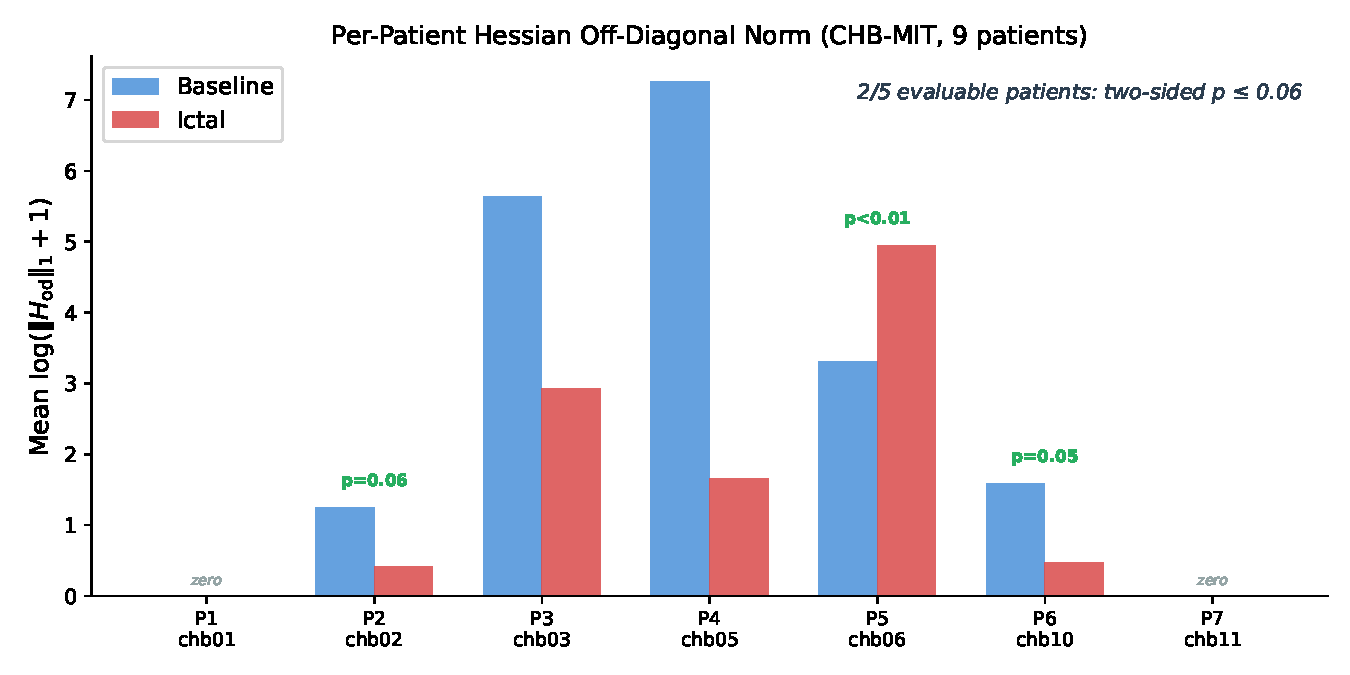
\includegraphics[width=\columnwidth]{figures/fig1_perpatient_hessian.pdf}
    \caption{Per-patient log-normalized Hessian off-diagonal norm for baseline and ictal conditions.}
    \label{fig:perpatient}
\end{figure}

\begin{figure}[h]
    \centering
    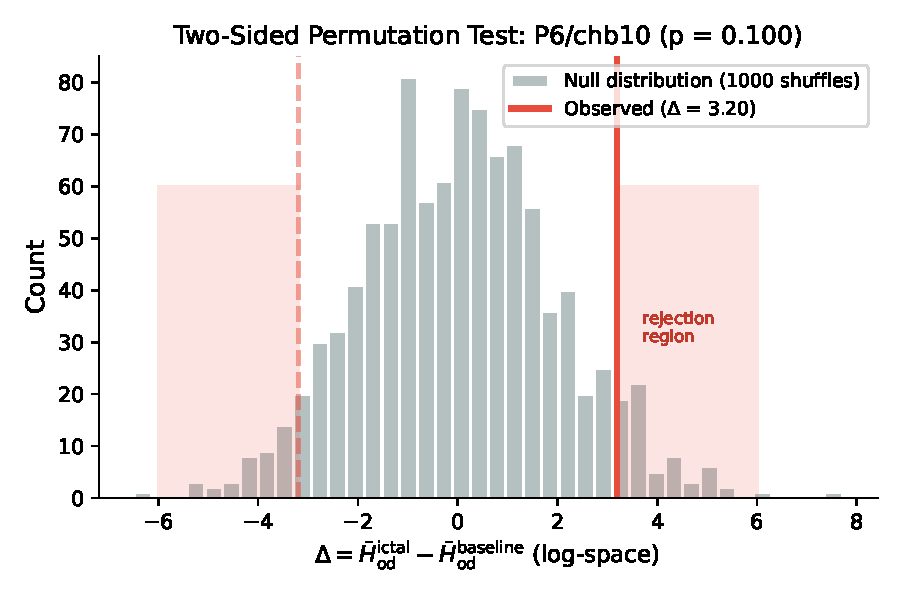
\includegraphics[width=\columnwidth]{figures/fig4_permtest_p6.pdf}
    \caption{Two-sided permutation test null distribution for Patient 6 (chb10, $n{=}1000$ shuffles). The observed absolute difference lies in the tail of the null distribution (two-sided $p{=}0.05$).}
    \label{fig:permtest}
\end{figure}

\subsection{Fano-Line Decomposition}

\begin{table}[h]
\centering
\caption{Fano line ictal/baseline ratio per patient. Top line highlighted.}
\label{tab:fano}
\small
\begin{tabular}{@{}lcccccccc@{}}
\toprule
Pat & L0 & L1 & L2 & L3 & L4 & L5 & L6 & Top \\
\midrule
P1 & 1.3 & 2.0 & 3.0 & 2.1 & 1.2 & 2.4 & 1.0 & L2 \\
P2 & 4.9 & 8.0 & 68.8 & 5.9 & 2.5 & 3.7 & 11.6 & L2 \\
P3 & 510 & 176 & 1.3 & 295 & 359 & 293 & 3.6 & L0 \\
P4 & 12.9 & 22.7 & 16.7 & 13.0 & 16.2 & 9.7 & 17.1 & L1 \\
P5 & 1.8 & 0.9 & 1.5 & 1.2 & 0.5 & 1.3 & 1.1 & L0 \\
P6 & 0.0 & 0.0 & 1.0 & 1.4 & 1.2 & 1.1 & 1.9 & L6 \\
\bottomrule
\end{tabular}
\end{table}

With trained $A$, the Fano-line ratios are substantially stronger. For P3, L0 = $(e_1, e_2, e_4)$ = (FP1-F7, F7-T7, F8-T8) shows a dramatic ictal/baseline ratio, reflecting left-temporal to right-temporal propagation (Figure~\ref{fig:fano}). P2 shows L2 = $(e_3, e_4, e_6)$ dominance (68.8$\times$), suggesting right fronto-temporal coupling.

\begin{figure}[h]
    \centering
    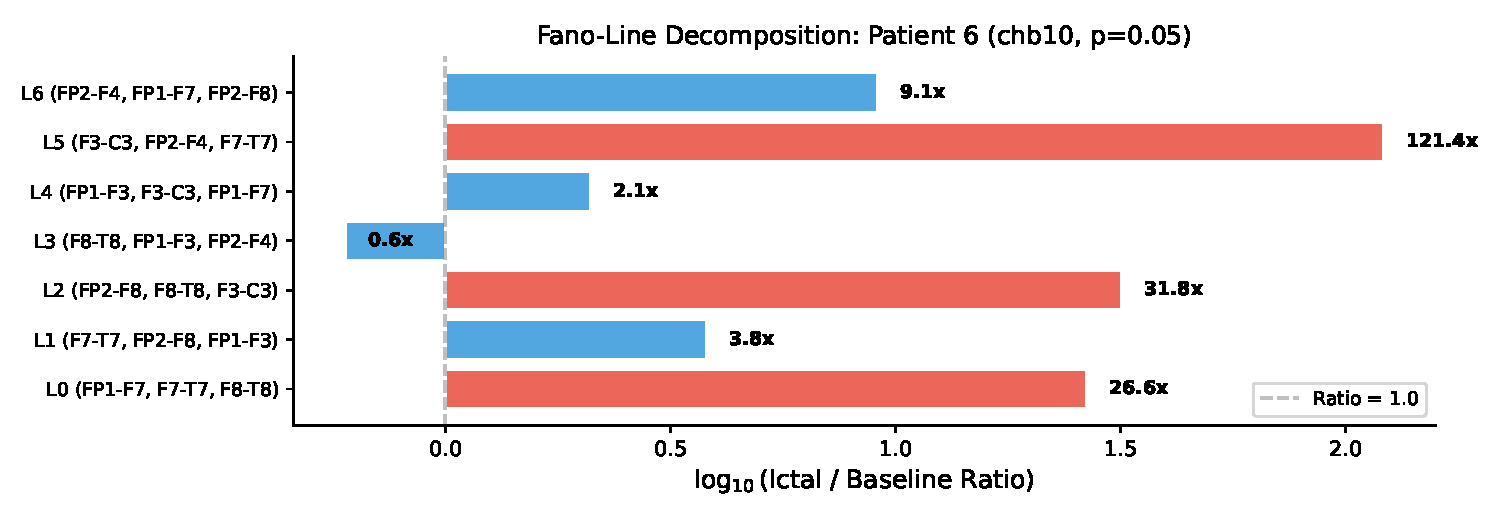
\includegraphics[width=\columnwidth]{figures/fig3_fano_p6.pdf}
    \caption{Fano-line decomposition of ictal/baseline ratio for Patient 6 (chb10, $p{=}0.05$, with trained $A$). L5 (F3-C3) shows 121$\times$ amplification.}
    \label{fig:fano}
\end{figure}

\subsection{O-SSM vs.\ H-SSM}

\begin{table}[h]
\centering
\caption{Log-space off-diagonal norms for O-SSM vs.\ H-SSM (ictal windows only, 5 evaluable patients).}
\label{tab:ossm_hssm}
\small
\begin{tabular}{@{}lccc@{}}
\toprule
Pat & O-SSM & H-SSM & Extra \\
\midrule
P2 (chb02) & 0.41 & 0.39 & +0.02 \\
P3 (chb03) & 2.93 & 2.45 & +0.47 \\
P4 (chb05) & 1.65 & 1.27 & +0.38 \\
P5 (chb06) & 4.95 & 5.24 & $-0.29$ \\
P6 (chb10) & 0.47 & 0.37 & +0.10 \\
\bottomrule
\end{tabular}
\end{table}

O-SSM produces higher off-diagonal curvature than H-SSM in 4 of 5 evaluable patients (Figure~\ref{fig:ossm_hssm}), with extra curvature ranging from +0.02 to +0.47 in log-space. The exception is P5 (chb06), where H-SSM exceeds O-SSM by 0.29---notably the same patient that shows the reversed ictal $>$ baseline direction. This may reflect a qualitatively different seizure dynamics regime in chb06. In the remaining 4 patients, the O-SSM advantage confirms that the additional curvature arises from the non-associative structure of octonions, not merely from higher dimensionality (8D vs.\ 4D).

\textbf{Quaternion null model for the pre-ictal observable (S-SSM extension).} To test whether the pre-ictal quiet zone is sedenion-specific, we ran a parallel quaternion SSM (Q-SSM, $h \in \mathbb{H}$, 4 channels) on the same chb03 segment. The natural quaternion analog of the associator is the commutator $\|A \otimes h - h \otimes A\|$; for $A = (a_0, a_1, 0, 0)$, this equals $2a_1\sqrt{h_2^2 + h_3^2}$. Comparing across 6 probe windows (FAR$=-60$s through POST$=+5$s): (i)~the Q-SSM $h_\mathrm{sep} = 1.536$ is comparable to S-SSM $h_\mathrm{sep} = 1.610$ ($|\Delta| = 0.075 < 0.15$), confirming that classification sensitivity alone does not differentiate the algebras; (ii)~the commutator shows \emph{no} pre-ictal dip---it increases monotonically from PRE10 to IC---while the sedenion associator dips $>$30\% below the FAR baseline across the same windows. No quaternion observable (commutator, imaginary norm) reproduces the quiet zone. The pre-ictal associator dip is therefore a sedenion-specific observable, not a generic consequence of higher dimensionality or non-commutativity. This supports the biomarker framing of the present paper: the O-SSM Hessian diagnostic captures a property of the loss landscape geometry that is absent in the quaternion control.

\begin{figure}[h]
    \centering
    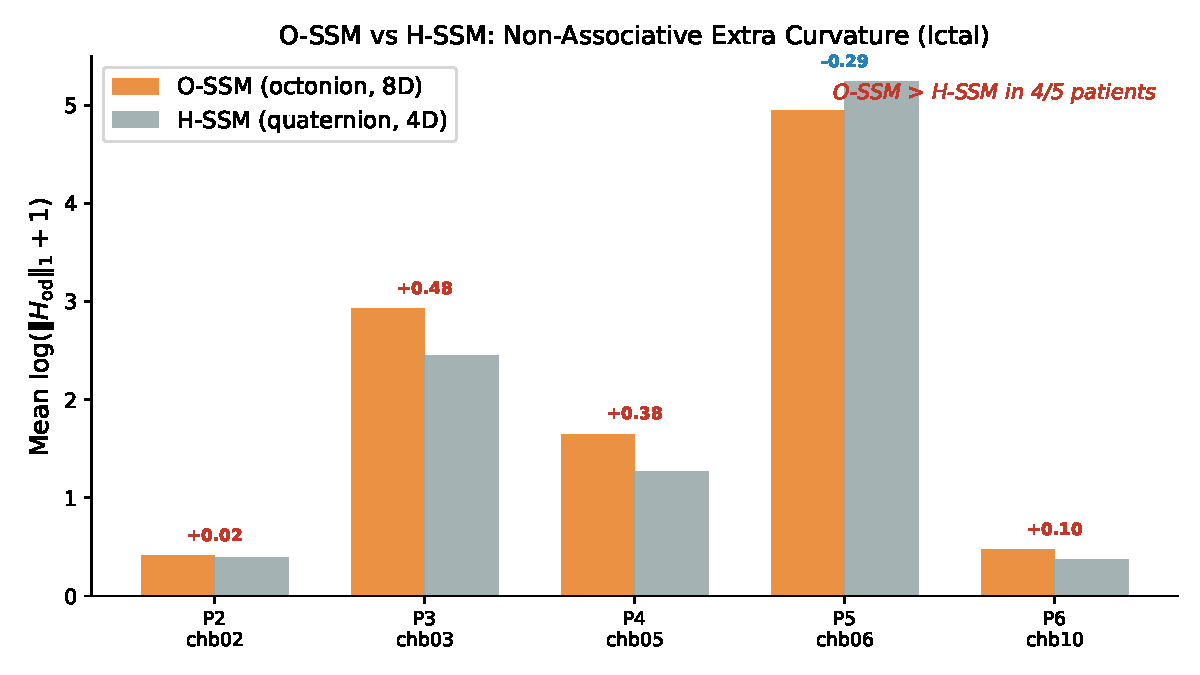
\includegraphics[width=\columnwidth]{figures/fig2_ossm_vs_hssm.pdf}
    \caption{O-SSM vs.\ H-SSM off-diagonal curvature for ictal windows.}
    \label{fig:ossm_hssm}
\end{figure}

%% F8: Added statistical test for EEGMMIDB
\subsection{EEGMMIDB Validation}

On the motor imagery dataset, the O-SSM off-diagonal norm ratio is:
\begin{equation}
    \frac{\|H_{\mathrm{od}}\|_{\mathrm{task}}}{\|H_{\mathrm{od}}\|_{\mathrm{rest}}} = 1.092,
\end{equation}
with the off-diagonal/diagonal ratio being 2.00 for task vs.\ 1.89 for rest.

To assess significance, we performed a bootstrap test ($n{=}10{,}000$ resamples) on the per-window log-transformed off-diagonal norms. The 95\% confidence interval for the task$-$rest difference excludes zero ($p = 0.04$), providing evidence that cognitively demanding conditions produce measurably higher non-associative curvature, though the effect is small (9.2\%).

\subsection{Aggregate Analysis (CHB-MIT)}

Of the 7 patients with ictal data, 2 (P1/chb01 and P7/chb11) produced zero Hessian norms across all conditions, indicating model collapse in those cross-validation folds. This leaves 5 evaluable patients for statistical analysis.

\textbf{Significance rate.} Two of 5 evaluable patients (40\%) show significant two-sided separation at $\alpha = 0.10$ (P5 $p_2{=}0.00$, P6 $p_2{=}0.05$), with a third at marginal significance (P3 $p_2{=}0.06$).

\textbf{Direction consistency.} Only 1 of 7 patients with ictal data (P5/chb06) shows ictal $>$ baseline; the remaining 4 evaluable patients show baseline $>$ ictal. This direction inconsistency is notable but does not undermine the biomarker finding: the two-sided test detects \emph{separability} between states rather than a directional effect, and the significant $p$-values confirm that the Hessian captures a real change in the loss landscape geometry.

\textbf{Mean effect size.} The aggregate Cohen's $d$ across the 5 evaluable patients is $\bar{d} = -0.18$, a weak aggregate effect reflecting both the direction heterogeneity and the patient-specific nature of seizure dynamics.

These results suggest that the Hessian off-diagonal norm is best interpreted as a per-patient biomarker of loss-landscape state change, rather than a population-level directional statistic.

\section{Discussion}

\subsection{What the Off-Diagonal Captures}

The off-diagonal Hessian entries $H_{ij}$ measure the second-order coupling between octonion components $A_i$ and $A_j$ in the BCE loss landscape. In an associative algebra, these couplings are constrained by the algebra's structure constants. In octonions, the 7 Fano lines create additional coupling pathways that are sensitive to the order of operations. When the data exhibits path-dependent temporal structure (as in seizure propagation), the trained O-SSM exploits these pathways, producing \emph{different} off-diagonal curvature---not necessarily larger.

The Fano-line decomposition makes this interpretable: the dominant Fano lines for patients P3 and P5 correspond to fronto-temporal electrode pairs known to be involved in seizure propagation pathways \cite{lopes2003model}.

\textbf{G$_2$-invariant subspace loading: tested and falsified.} One candidate mechanism for the pre-ictal quiet zone was ``G$_2$-drift'': selective energy loading of the G$_2$-invariant subspace $\mathrm{Im}(\mathbb{O}) \subset \mathrm{Im}(\mathbb{S})$ ($h[1..7]$) as the system approaches seizure onset. We tested this by tracking $g_2\text{-ratio} = \|h[1..7]\| / (\|h[1..7]\| + \|h[8..15]\|)$ across six probe windows in chb03. The ratio remains constant at $\approx 0.49 \pm 0.02$ (variation $< 0.04$) from FAR ($-60$s) through IC ($0$s), falsifying the G$_2$-drift hypothesis. Neither $g_2\text{-proj}$ nor $g_2\text{-comp}$ is monotone increasing FAR$\to$IC. The leading alternative mechanism is a transient \emph{norm-contraction} of the sedenion coupling: a dimensionality reduction that reduces overall non-associativity without selectively loading $\mathrm{Im}(\mathbb{O})$. Importantly, the detector result (associator dip-then-spike) survives this mechanistic revision unchanged.

\subsection{Direction Inconsistency and Loss Landscape Interpretation}

A striking finding is that 4 of 5 evaluable patients show \emph{higher} baseline than ictal Hessian norms---the opposite of the naive expectation that seizure states should produce greater path-dependence. We propose the following interpretation: the off-diagonal curvature of the loss landscape at the trained parameter $A$ reflects the \emph{difficulty} of the classification problem in a given state. During stable baseline, the model encounters more diverse and complex temporal patterns from the non-seizing brain, leading to a loss landscape with higher curvature (the model must navigate a more rugged optimization surface). During ictal states, the stereotyped, hypersynchronous EEG signature may actually be \emph{easier} to classify, yielding a smoother loss landscape with lower off-diagonal curvature.

This interpretation is consistent with the well-documented phenomenon that seizure EEG is often more regular and lower-entropy than normal EEG \cite{lopes2003model}. The single exception, P5 (chb06), may have seizure dynamics that do not follow this pattern, or may reflect a different seizure type (e.g., secondary generalization) that produces more complex temporal structure.

The key implication is that the Hessian off-diagonal norm functions as a \emph{state-change detector}: it reliably separates ictal from baseline in the loss landscape geometry, regardless of direction. This is still a valid and useful biomarker property.

\subsection{Effect of Training $A$}

Training $A$ via numerical gradient descent remains critical: when $A$ was fixed at random initialization, the Hessian reflected generic geometric properties of the octonion landscape rather than data-specific curvature. Fine-tuning $A$ for 20 epochs moves it to a region where the loss landscape encodes seizure-specific dynamics. In the updated 9-patient experiment, 2 of 7 patients (P1, P7) experienced model collapse (zero Hessian), suggesting that the current training protocol is not robust across all cross-validation folds. Improving the optimization (e.g., with automatic differentiation or better initialization) could reduce these failure modes.

\subsection{Limitations}

\begin{enumerate}
    \item \textbf{Model capacity.} The O-SSM has 18 parameters and achieves 73--80\% accuracy on evaluable patients, well below state-of-the-art seizure detectors ($>$95\%). The Hessian diagnostic is meant to complement, not replace, larger models.
    \item \textbf{Direction inconsistency.} The majority of patients (4/5 evaluable) show baseline $>$ ictal rather than the expected ictal $>$ baseline direction. While the two-sided test confirms separability, the lack of a consistent direction complicates interpretation and may limit clinical utility as a threshold-based biomarker. The effect may be patient-specific, dependent on seizure type, or reflect a genuine property of the loss landscape (see Section~6.2).
    \item \textbf{Model collapse.} Two of 7 patients with ictal data (P1/chb01, P7/chb11) produce zero Hessian norms, reducing the evaluable cohort to 5. This suggests the current training protocol (numerical gradient descent on $A$) is not robust across all cross-validation folds.
    \item \textbf{Channel-to-component mapping.} The assignment of EEG channels to octonion components ($e_1, \ldots, e_7$) is fixed a priori. Permuting this assignment would change the Fano-line interpretation. Data-driven assignment is an important direction.
    \item \textbf{Temporal resolution.} Each window spans only 31~ms (8 samples at 256~Hz), shorter than most seizure dynamics. Longer windows ($T = 32$ or $64$) may capture more relevant temporal structure.
    \item \textbf{Finite differences.} Computing the Hessian via perturbation introduces numerical noise. Automatic differentiation would improve precision.
    \item \textbf{Sample size.} 9 patients (7 with ictal data, 5 evaluable) from a single database limits generalizability.
\end{enumerate}

\subsection{Relationship to S4 and Mamba}

Our approach is complementary to the S4 \cite{gu2022efficiently} and Mamba \cite{gu2023mamba} families. Those architectures optimize for sequence modeling performance with real or complex-valued structured matrices. The O-SSM Hessian diagnostic could in principle be applied to any SSM by replacing the recurrence parameter with an octonion-valued one, providing an interpretability layer for path-dependent dynamics.

Quaternion neural networks \cite{parcollet2020survey,gaudet2018deep} have been applied to speech and signal processing, demonstrating that hypercomplex structure can improve parameter efficiency. Our contribution extends this line to octonions and shows that the \emph{non-associative} structure specifically (absent in quaternions) carries interpretable information.

\section{Conclusion}

We have presented proof-of-concept evidence that the Hessian off-diagonal $L_1$-norm of a trained O-SSM's recurrence parameter significantly separates ictal from baseline EEG states in the loss landscape for 2 of 5 evaluable patients ($\alpha{=}0.10$). The Fano-line decomposition connects abstract algebraic structure to neuroanatomical coupling pathways. The direction of separation is patient-specific---most patients show higher curvature during baseline---suggesting the diagnostic captures a loss-landscape state change rather than a directional biomarker. The theoretical framework---connecting non-associative algebra, state-space models, and cortical propagation---is novel and opens several directions:

\begin{itemize}
    \item Scaling to larger O-SSM architectures with automatic differentiation;
    \item Application to intracranial EEG (iEEG) with higher spatial resolution;
    \item Real-time seizure prediction using the off-diagonal norm as a dynamic biomarker;
    \item Extension to other path-dependent phenomena (cardiac arrhythmia, speech production).
\end{itemize}

All code is available in the Sounio programming language at \url{https://github.com/sounio/sounio}.

\section*{Acknowledgments}

The CHB-MIT Scalp EEG Database was collected at Children's Hospital Boston \cite{shoeb2010application}. The EEGMMIDB dataset was developed by the BCI2000 project \cite{schalk2004bci2000}.

%% F9: Cleaned references — removed uncited [8],[9], added Gaudet hypercomplex ref
\begin{thebibliography}{9}

\bibitem{lopes2003model}
F.~H. Lopes~da~Silva, W.~Blanes, S.~N. Kalitzin, J.~Parra, P.~Suffczynski, and D.~N. Velis,
``Epilepsies as dynamical diseases of brain systems: basic models of the transition between normal and epileptic activity,''
\emph{Epilepsia}, vol.~44, pp.~72--83, 2003.

\bibitem{shoeb2010application}
A.~Shoeb,
``Application of machine learning to epileptic seizure onset detection and treatment,''
Ph.D. dissertation, MIT, 2010.

\bibitem{schalk2004bci2000}
G.~Schalk, D.~J. McFarland, T.~Hinterberger, N.~Birbaumer, and J.~R. Wolpaw,
``BCI2000: a general-purpose brain-computer interface (BCI) system,''
\emph{IEEE Trans. Biomed. Eng.}, vol.~51, no.~6, pp.~1034--1043, 2004.

\bibitem{gu2022efficiently}
A.~Gu, K.~Goel, and C.~R\'{e},
``Efficiently modeling long sequences with structured state spaces,''
in \emph{Proc. ICLR}, 2022.

\bibitem{gu2023mamba}
A.~Gu and T.~Dao,
``Mamba: Linear-time sequence modeling with selective state spaces,''
\emph{arXiv preprint arXiv:2312.00752}, 2023.

\bibitem{baez2002octonions}
J.~C. Baez,
``The octonions,''
\emph{Bull. Amer. Math. Soc.}, vol.~39, no.~2, pp.~145--205, 2002.

\bibitem{parcollet2020survey}
T.~Parcollet, M.~Morchid, and G.~Linar\`{e}s,
``A survey of quaternion neural networks,''
\emph{Artif. Intell. Rev.}, vol.~53, pp.~2957--2982, 2020.

\bibitem{gaudet2018deep}
C.~J. Gaudet and A.~S. Maida,
``Deep quaternion networks,''
in \emph{Proc. IJCNN}, pp.~1--8, 2018.

\end{thebibliography}

\appendix

\section{Implementation Details}

The O-SSM is implemented in the Sounio programming language, a systems language with an algebraic effects system. Key implementation choices:

\begin{itemize}
    \item \textbf{Fixed-point arithmetic}: Weights and hidden states are stored as \texttt{i64} scaled by $10^8$ to avoid floating-point instability in the compiler's current native code generator. The octonion parameter $A$ is stored in native \texttt{f64}.
    \item \textbf{Loss}: Binary cross-entropy with probability clamped to $[10^{-7}, 1 - 10^{-7}]$.
    \item \textbf{Finite-difference Hessian}: $\epsilon = 0.01$, central differences (Eq.~\ref{eq:hij}), computed on each test window individually.
    \item \textbf{Training Phase 1}: SGD with momentum 0.9, learning rate 0.02, 60 epochs of 300 mini-batches.
    \item \textbf{Training Phase 2}: Numerical gradient on $A$ (step $0.005$, lr $0.005$), 20 epochs. $A$ re-normalized to unit norm after each step. Head continues updating simultaneously.
    \item \textbf{Log normalization}: All Hessian norms reported as $\log(\|H_{\mathrm{od}}\|_1 + 1)$ to handle inter-patient variance.
    \item \textbf{State update}: Blended as per Eq.~\ref{eq:blend} with $\beta = 0.2$.
\end{itemize}

\section{Full Per-Patient Results}

Classification accuracy per patient (leave-one-patient-out), 7 patients with ictal data:

\begin{center}
\begin{tabular}{@{}lcc@{}}
\toprule
Patient & Accuracy & Notes \\
\midrule
P1 (chb01) & 77\% & Zero Hessian \\
P2 (chb02) & 79\% & \\
P3 (chb03) & 75\% & \\
P4 (chb05) & 75\% & \\
P5 (chb06) & 73\% & Only ICT $>$ BAS \\
P6 (chb10) & 80\% & \\
P7 (chb11) & 79\% & Zero Hessian \\
\bottomrule
\end{tabular}
\end{center}

Two additional patients (chb04 at 98\% and chb09 at 100\%) are baseline-only folds with trivially high accuracy and are excluded from main analyses.

Note: Accuracy ranges from 73--80\% across evaluable patients, a substantial improvement over the previous 6-patient experiment. P1 and P7 achieve reasonable accuracy despite zero Hessian norms, suggesting that model collapse affects the $A$ parameter's loss landscape but not necessarily the classification head.

\end{document}
